\documentclass{article}

\textwidth=6.5in
\textheight=8.5in
\voffset=-54pt
\oddsidemargin=0in
\evensidemargin=0in
\setlength{\parskip}{8pt}
\setlength{\parindent}{0pt}

\usepackage{amsmath, amssymb}
\usepackage{ifthen}

\usepackage[inline]{enumitem}
\setlist{topsep=0pt, parsep=8pt}

\usepackage[rgb,table]{xcolor}\convertcolorsUfalse
\usepackage{graphicx}

% change hyperref options
\PassOptionsToPackage{hyphens}{url}
\usepackage[bookmarks,colorlinks,linkcolor=black,citecolor=blue,pdfstartview=FitH,urlcolor=blue]{hyperref}
\hypersetup{pdfpagemode=UseNone}
\usepackage{bookmark}

\usepackage{graphicx}
\usepackage{multicol}
\usepackage{framed}
\usepackage{array}

\usepackage{icomma}

\usepackage{marginnote}
\usepackage[colorinlistoftodos]{todonotes}
\renewcommand{\marginpar}{\marginnote}

\usepackage{soul}

\usepackage{tikz}
\usetikzlibrary{
  matrix,%
  % enables the snake paths
  decorations.pathmorphing,%
  % enables bigger arrows
  decorations.markings,%
  decorations.pathreplacing,%
  decorations.text,%
  calc,%
  patterns,%
  shapes.geometric,%
  arrows,
  decorations.shapes,
  positioning,
  plotmarks,
  intersections
}
\tikzset{>=latex} % sets default arrow type in tikz
\tikzset{font=\normalsize}
\tikzset{mark size=1.5pt, mark options=thin}
\tikzset{pin distance=4pt,
  every pin edge/.style={<-, thin, shorten <= -2pt}}

\interfootnotelinepenalty=10000
\renewcommand{\thefootnote}{(\arabic{footnote})}

\usepackage{multirow, bigdelim}

% change to \usepackage[sols]{handout} to see solutions
\usepackage[]{handout}
\renewcommand{\workshopnote}{CA Notes.}    

\newcommand\iscurrentenumi[1]{%
  \ifthenelse{\equal{#1}{\theenumi}}{}{#1}}
\setenumerate[1]{ref=\#\arabic*}
\setenumerate[2]{ref=\protect\iscurrentenumi{\theenumi}(\alph*)}
\newcommand\enumiiprefix[2]{%
  \ifthenelse{{\equal{#1}{\theenumi}}\AND{\equal{#2}{(\alph{enumii})}}}{}{}%
  \ifthenelse{{\equal{#1}{\theenumi}}\AND{\NOT{\equal{#2}{(\alph{enumii})}}}}{#2}{}%
  \ifthenelse{\equal{#1}{\theenumi}}{}{#1#2}%
}
\setenumerate[3]{ref=\protect\enumiiprefix{\theenumi}{(\alph{enumii})}\roman*}

\definecolor{purple}{rgb}{0.5,0,1.0}
\definecolor{skyblue}{rgb}{0, 0.5, 1}

\newcommand{\highlight}[1]{\boldmath\hl{\textbf{#1}}\unboldmath}

\newcommand{\goal}[1]{\textbf{\textcolor{skyblue}{#1}}}

\newcommand{\doedfinity}[2][\newpage]{
  \begin{problem}[#1]
    Do the Edfinity assignment ``Problem Set #2''.

    We encourage you to write down any scratch work here, as well as
    things you want your future self to remember. Nothing you write
    here will be graded; it's just for you!
  \end{problem}
}

\newcommand{\psrnewpage}{\newpage}
\newcommand{\psreflection}[2][]{

  \ifthenelse{\not\equal{#1}{nocite}}{
    \begin{enumerate}[resume]
    \item
      \begin{problem}[1in]
        Please cite any help you got on this problem set:
        \begin{itemize}[nosep]
        \item If you worked with other students, please list their names here.
        \item If you used resources other than those on our Canvas site, please list them here.
        \end{itemize}
      \end{problem}

    \end{enumerate}
  }

  \probonly{%
    #2

    \psrnewpage

    \emph{Reflection space.} It's a good habit to take a few minutes at the end of each pset to reflect on what you learned and jot down notes to your future self. Here are a few reflection questions to get you started. Nothing you write here will be graded; it's just for you!
    \begin{itemize}
    \item Take a few minutes to look back at the problems. How could you explain to someone else how to do each problem? What was your strategy, and how did you know to use that strategy? If there are problems where you don't feel able to answer this, write down which ones they are. Come back to them in a few days when we post the homework solutions!

      \vspace{1.5in}

    \item Take a look back at the learning objectives on today's worksheet; how are you feeling about each one? If there are ones you know you need more practice with, write those down here.

      \vspace{1.5in}

    \item What did you find most challenging about this material? Do you have any lingering questions about it? If so, write them down here so you don't forget them. At some point, stop by office hours or MQC to ask!

      \vfill
    \end{itemize}      
  }
}

\usepackage{fancyhdr}
\lhead{\textcolor{white}{This content is protected and may not be shared, uploaded, or distributed.}}
\rhead{}
\rfoot{\vspace*{\fill}\footnotesize\textcopyright{} \emph{Harvard Math Ma}}
\renewcommand{\headrulewidth}{0pt}
\pagestyle{fancy}
\begin{document}

\begin{center}
  \large\textsc{Problem Set 22 - Optimization}\vspace{.5in}\\
  \begin{problemonly}
   \large Name: \rule{5cm}{0.15mm}\\
   \end{problemonly}
\end{center}


\begin{workshop}
  The easiest step for students to forget is that they need to use some sort of reasoning (the First Derivative Test, Second Derivative Test, or plugging the critical points and endpoints into the function) to justify that they've actually found the global minimum or maximum (rather than just a critical point).
\end{workshop}

For full credit on optimization problems, please do the following in each problem:
{
  \begin{itemize}[nosep]
  \item State the goal (like ``Minimize cost'').
  \item If the problem involves some geometry, draw a picture, and label both variables and constants on your picture. If the problem doesn't involve geometry, use words to explain each variable you use (like ``$b$ = number of bowls sold'').
  \item Clearly communicate your thought process, one step at a time. Write down how you find the global maximum or minimum, and \textbf{justify that it really is a global maximum or minimum}. 
  \item Be sure to answer the original question!
  \end{itemize}
}

\begin{center}
  \rule{5in}{0.4pt}
\end{center}

\begin{enumerate}
\item \label{spring2011-midterm1-revisit-5}

  \begin{grading}
    10 points:
    \begin{itemize}[nosep]
    \item 1 for stating the goal
    \item 1 for labeling the picture
    \item 1 for having a correct formula for the area in terms of whatever variables they've labeled
    \item 2 for correctly using the fact that the perimeter is 30 to get the area in terms of one variable
    \item 2 for correctly finding the critical point of their area function
    \item 2 for justifying that the critical point is a global max. They can use the First Derivative Test, Second Derivative Test, or end behavior. If they use the FDT or SDT, technically they should say there's only one critical point. Otherwise, they've only shown it's a local max / min, not a global one. If they omit this, please give them feedback and deduct 0.01 (just so they know there's some feedback). 
    \item 1 for answering the question (that is, giving both dimensions of the window)
    \end{itemize}
  \end{grading}

  \begin{problem}[\newpage]
    A Norman window has the shape of a semicircle on top of a rectangle. (The diameter of the semicircle is equal to the width of the rectangle.) If the perimeter of the window must be 30 feet, find the dimensions of the window so that the greatest possible amount of light is admitted. (Assume the bigger the area of glass, the more light is admitted.)

    In the picture below, the gray area is all glass. The perimeter is the heavy dark line.

    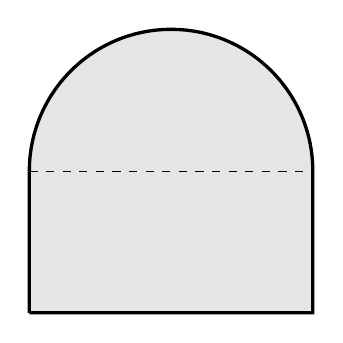
\begin{tikzpicture}[x=1.8cm, y=1.8cm]
      \filldraw[fill=black!10!white, very thick] (0, 0) -- (2, 0) -- (2, 1) arc[radius=1, start angle=0, end angle=180] -- (0, 0); %
      \draw[dashed] (0, 1) -- (2, 1); % 
    \end{tikzpicture}
  \end{problem}

  \begin{solution}
    \highlight{Goal:} Maximize \goal{area}.

    \highlight{Define variables:}
    Let $r$ be the radius of the semicircle, $h$ be the height of the rectangle, $A$ be the
    total area of the window.
    \begin{center}
      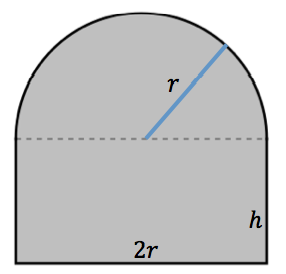
\includegraphics[width=150px]{images/window.png}
    \end{center}
    \highlight{Formula for goal:} $\goal{$A$} = \frac{1}{2}\pi r^2 + 2rh$.

    We need to \highlight{relate $r$ and $h$ using information from the problem.}
    We are told that the total perimeter is 30 feet. So, 
    \begin{align*}
    \frac{1}{2}(2\pi r)+2h+2r &= 30\\
    (\pi+2)r+2h &= 30 \\
    h &= 15 - \tfrac{1}{2}(\pi+2)r
    \end{align*}

    So our function is
    \[A(r) = \tfrac{1}{2}\pi r^2 + 2r[15-\tfrac{1}{2}(\pi +2)r]
    = 30r - (\tfrac{\pi}{2} +2)r^2\]
    There are no bounds for $r$ given in the problem, so we need to work off of the
    constraint that the perimeter is 30 feet. The lower bound for $r$ is zero, which
    corresponds to $h=15$. The upper bound for $r$ is attained when $h$ is at
    its lower bound, zero.
    \begin{align*}
      (\pi +2)r + 2(0) &= 30\\
      r &= \frac{30}{\pi + 2}
    \end{align*}
    So the domain is $0 \leq r \leq \frac{30}{\pi+2}$.

    \highlight{Critical points:} Now we need to find the critical points on the domain.
    $A'(r)=30-(\pi + 4)r$, so
    \begin{align*}
      30 - (\pi + 4)r &= 0 \\
      r &= \frac{30}{\pi + 4}
    \end{align*}
    This is the only critical point on the domain.

    \highlight{Global maximum:} Since there is only one critical point on the domain, if
    we can show that it is a local maximum, then it is the global maximum. We'll use
    the Second Derivative Test. $A''(r) = -(\pi + 4)$, so $A''(\frac{30}{\pi+4})$ is negative,
    and thus $A(r)$ achieves its global maximum at $r=\frac{30}{\pi + 4}$.

    \highlight{Answer the question:} The global maximum is at $r=r=\frac{30}{\pi + 4}$.
    Plugging this back into the perimeter constraint, we can find that this
    corresponds to a height of $h=15-\frac{1}{2}(\pi+2)(\frac{30}{\pi +4}) = 
    \frac{30}{\pi + 4}$. So, the most light is admitted when 
    \fbox{the radius and height are both
    $\frac{30}{\pi+4}$ feet}.
  \end{solution} 

\item \label{optimization-fence}

  \note{The critical point is a local minimum, so they need to test the endpoints.}

  \begin{workshop}
    It's easy for students to assume that the critical point must be the extremum we're looking for. Don't immediately let them know if they've made that mistake here; \ref{optimization-reflect-back} is meant to help students realize this.
  \end{workshop}

  \begin{grading}
    7.5 points:
    \begin{itemize}[nosep]
    \item 1 for stating the goal
    \item 1 for defining their variables clearly, either in a picture or in words
    \item 0.5 for having a correct formula for the perimeter in terms of whatever variables they've defined
    \item 1 for correctly using the fact that the area is 400 to get the perimeter in terms of one variable
    \item 1 for correctly finding the critical point of their perimeter function 
    \item 2 for finding the actual global maximum and justifying it 
    \item 1 for answering the question
    \end{itemize}
  \end{grading}

  \begin{problem}[\newpage]
    A fence company has decided to construct a small public garden to show off their fence to potential customers. The garden will have an area of 400 square feet, and it needs to be at least 10 feet long and 10 feet wide. The company would like to maximize the perimeter of the garden so that they can show off as much fence as possible. What dimensions should they make the garden? 
  \end{problem}

  \begin{solution}
    \highlight{Goal:} Maximize \goal{perimeter}.

    \highlight{Define variables:}
    \begin{itemize}[nosep]
      \item $\ell$ = length of rectangular garden
      \item $w$ = width of rectangular garden
      \item $P$ = perimeter of rectangular garden
    \end{itemize}
    \begin{center}
      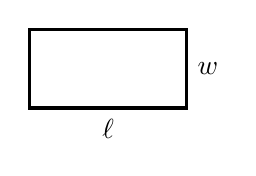
\begin{tikzpicture}
        \draw[very thick] (0,0) -- node[midway, below] {$\ell$} (2,0) -- node[midway, right]
        {$w$} (2,1) -- (0, 1) -- cycle;
      \end{tikzpicture}
    \end{center}
    \highlight{Formula for goal:} $\goal{$P$} = 2\ell + 2w$

    To get this as a function of only one variable, we need to 
    \highlight{relate $\ell$ and $w$ using information from the problem.} We're told
    that the garden has an area of 400 square feet, so $\ell w =400$, and 
    $w = \frac{400}{\ell}$.
    Therefore our function is
    \[P(\ell) = 2\ell + 2\left(\frac{400}{\ell}\right) = 2\ell + \frac{800}{\ell}.\]
    We're told that the lower bound for $\ell$ is $10$ feet. Since the area is constant,
    the upper bound for $\ell$ is attained when $w$ is at its lower bound:
    \begin{align*}
        \ell (10) &= 400 \\
        \ell &= 40
    \end{align*}
    Therefore the domain is $10 \leq \ell \leq 40$.

    \highlight{Critical points:} Now we need to find the critical points on the domain.
    $P'(\ell) = 2 - \frac{800}{\ell^2}$, so
    \begin{align*}
      2 - \frac{800}{\ell^2} &= 0 \\
      \frac{2\ell^2 - 800}{\ell^2} &= 0 \\
      2\ell^2 - 800 &= 0 \\
      \ell^2 &= 400 \\
      \ell &= \pm 20
    \end{align*}
    Since the domain is $10 \leq \ell \leq 40$, the only critical point is $\ell = 20$.

    \highlight{Global maximum:} Since there's only one critical point, if it's
    a local maximum, then it will be the global maximum. Let's try to use the First Derivative
    Test. The sign chart for $P'(\ell)$ on $[10, 40]$ looks like this:
      \begin{center}
        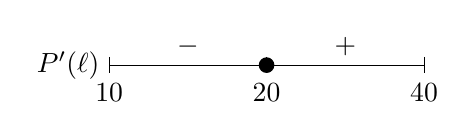
\begin{tikzpicture}
          \draw[-] (-2,0) -- (2, 0);
          \node[left] at (-2,0) {$P'(\ell)$};
            \draw[shift={(-2,0)},color=black] (0pt,3pt) -- (0pt,-3pt) node[below] {$10$};
            \draw[shift={(0,0)},color=black] (0pt,3pt) -- (0pt,-3pt) node[below] {$20$};
            \draw[shift={(2,0)},color=black] (0pt,3pt) -- (0pt,-3pt) node[below] {$40$};
            \node[circle, fill=black, inner sep=2pt] at (0,0) {};
          \node[above] at (-1,0) {$-$};
          \node[above] at (1,0) {$+$};
        \end{tikzpicture}
      \end{center}
      This shows that $\ell=20$ is a local minimum, not a local maximum. We therefore know
      that the global maximum must occur at one of the endpoints. Comparing the values,
      we find that
      \begin{align*}
        P(10) = 100 \\
        P(40) = 100
      \end{align*}
      so the global maximum is achieved at both $\ell = 10$ and $\ell = 40$. These
      correspond to $w=40$ and $w=10$, respectively.
      (This makes sense, because we arbitrarily chose which side to call $\ell$ 
      and which side to call $w$, and the rectangle is symmetric.)

      \highlight{Answer the question:} To maximize the perimeter, the company should make the
      dimensions of the garden \fbox{10 feet by 40 feet}.
  \end{solution}

\item % 10.3.14 modified

  \begin{grading}
    11 points:
    \begin{itemize}[nosep]
    \item 1 for stating the goal
    \item 1 for drawing and labeling a picture
    \item 3 for having a correct formula for the cost: 1 for correctly handling the fact that the top and bottom cost 3 times as much, 1 for surface area of the sides, 1 for surface area of the two squares
    \item 1 for correctly using the fact that the volume is 192 to get the cost in terms of 1 variable
    \item 2 for finding critical points of their cost function
    \item 2 for justifying that the critical point is a global min. They can use the First Derivative Test, Second Derivative Test, or end behavior. If they use the FDT or SDT, technically they should say there's only one critical point. Otherwise, they've only shown it's a local max / min, not a global one. If they omit this, please give them feedback and deduct 0.01 (just so they know there's some feedback). 
    \item 1 for answering the question (that is, giving both dimensions)
    \end{itemize}
  \end{grading}

  \begin{problem}[\newpage]
    A company is designing a can for mandarin oranges. The can will be a cylinder with a volume of 192 cubic centimeters. The metal used for the top and bottom is stronger than that used for the sides, so the metal for the top and bottom costs 3 times as much per square cm as the metal used for the sides.

    There is wasted metal in constructing the top and bottom because they need to be cut from squares of metal (as shown in the picture below), and the company must pay for the entire squares of metal. If the company wants to minimize the cost of the metal they spend on each can, what dimensions should they make the can?

    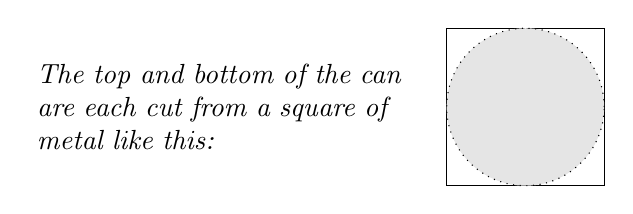
\begin{tikzpicture}
      \draw (-1, -1) rectangle (1, 1); %
      \filldraw[dotted, fill=black!10!white] (0, 0) circle(1);%
      \draw (-1, 0) node[left, text width=2in] {\emph{The top and bottom of the can are each cut from a square of metal like this:}};
    \end{tikzpicture}
  \end{problem}

  \begin{solution}
    \highlight{Goal:} Minimize the \goal{cost of a can.}

    \highlight{Define variables:} he can is pictured below: the lighter material (top and bottom) is stronger than the darker material, but it must be cut from a square, as pictured on the right.
    \begin{center}
      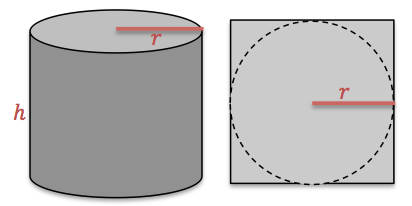
\includegraphics[width=200px]{images/orange-can.png}
    \end{center}
    Let's write an equation in words first to figure out which variables we'll need.
    \begin{align*}
        \goal{cost of a can} &= \text{cost of top and bottom} + \text{cost of sides} \\
        &= (\text{price per area of stronger metal})
        (\text{area of squares for top and bottom})\\
        &\hspace{1em} + (\text{price per area of weaker metal})(\text{area of sides})
    \end{align*}
    
    Let $C$ be the cost of the can. Let $h$ be the height of the can and let $r$ be the
    radius of the can.  Let $P$ be a constant that represents
    the price per area of the weaker metal.
    
    \highlight{Formula for goal:} $\goal{$C$} = 3P\cdot2(2r)^2 + P\cdot2\pi rh$

    Now we need to \highlight{relate $r$ and $h$ using information from the problem.} We're
    told that the volume of the can must be 192 cubic centimeters, so
    \begin{align*}
      \pi r^2 h &= 192 \\
      h &= \frac{192}{\pi r^2}
    \end{align*}
    
    Substituting this into our formula for the cost, we get:
    \[C(r)=3P\cdot2(2r)^2+P\cdot2\pi r\left(\frac{192}{\pi r^2}\right)=24Pr^2+\frac{384P}{r}
    = 24P\left(r^2 + \frac{16}{r}\right).\]
    The lower bound of $r$ is zero, not including zero, since the volume of the
    can must be 192 cubic centimeters. We can make the radius as large as we want by making
    the height arbitrarily small. So the domain is $r \geq 0$, or $(0, \infty)$.
    
    \highlight{Critical points:} Now we need to find the critical points
    on the domain. $C'(r) = 24P(2r -\frac{16}{r^2})$, so
    \begin{align*}
      24P\left(2r - \frac{16}{r^2}\right) &= 0 \\
      2r - \frac{16}{r^2} &= 0 \\
      \frac{2r^3 - 16}{r^2} &= 0 \\
      2r^3 - 16 &= 0 \\
      r^3 &= 8 \\
      r &= 2
    \end{align*}
    $C'(r)$ is undefined when $r=0$, but $r=0$ isn't in the domain, so the
    only critical point is $r=2$. 

    \highlight{Global minimum:} Since this is the only critical point on the domain,
    if we can show that it is a local minimum, then it must be the global minimum. We'll
    use the Second Derivative Test. $C''(r) = 24P(2+\frac{32}{r^3})$, so $C''(2)$ is positive,
    and therefore $C(r)$ achieves its global minimum at $r=10$.

    \highlight{Answer the question:} The corresponding value of $h$ to $r=10$
    is $h=\frac{192}{\pi(10)^2}=\frac{48}{25\pi}$. To minimize cost, the company should
    design the can to have a \fbox{radius of $10$ centimeters} and a \fbox{height of
    $\frac{48}{25\pi}$ centimeters}.
  \end{solution}

\item \textbf{Reflect Back.}

  \begin{enumerate}
  \item
    \begin{problem}
      Which method did you use in each problem to show that you actually found the global maximum or minimum (as opposed to just finding a critical point)? You don't have to write up an answer here, but look back at each problem to make sure you justified this.

      (There is nothing to write for this part.) 
    \end{problem}

  \item \label{optimization-reflect-back}

    \begin{grading}
      1 point
    \end{grading}

    \begin{problem}[0.75in]
      In one problem on this problem set, the global extremum you were looking for happened at an endpoint of the domain; which problem?
    \end{problem}

    \begin{solution} % Jason Bland
      This happened in \ref{optimization-fence}.
    \end{solution}

  \end{enumerate}

\item  \note{A reminder of percent change in preparation for next class on exponentials.}

  Next class, percent change will be important. Today's Edfinity assignment is a review of that. 

  \doedfinity[\vfill]{22} 

\end{enumerate}
\psreflection{For next class, read \S 9.1, 9.2.}
\end{document}

